\documentclass[11pt]{article}
\usepackage[margin=1in]{geometry}
\usepackage{fontspec}
\usepackage{booktabs}
\usepackage{longtable}
\usepackage{array}
\usepackage{float}
\usepackage{placeins}
\usepackage{graphicx}
\usepackage[font=small,labelfont=bf]{caption}
\usepackage{natbib}
\usepackage{xurl}
\usepackage[hidelinks]{hyperref}
\usepackage{setspace}
\setstretch{1.15}
\graphicspath{{../figs/}}
% Generated by scripts/tables.R; do not edit.
\newcommand{\nItems}{19}
\newcommand{\nPolls}{7}
\newcommand{\nRespondents}{1,988}
\newcommand{\nAnswers}{5,455}
\newcommand{\wrongBefore}{23\%}
\newcommand{\wrongAfter}{10\%}
\newcommand{\pooledChange}{12}
\newcommand{\pooledLower}{11}
\newcommand{\pooledUpper}{14}
\newcommand{\nFell}{11}
\newcommand{\nRose}{1}
\newcommand{\wrongToRight}{65\%}
\newcommand{\dkToRight}{62\%}
\newcommand{\rightDiff}{+1}
\newcommand{\rightDiffLower}{-4}
\newcommand{\rightDiffUpper}{+5}
\newcommand{\wrongToWrong}{24\%}
\newcommand{\dkToWrong}{12\%}
\newcommand{\wrongToDk}{12\%}
\newcommand{\dkToDk}{26\%}
\newcommand{\nStartWrong}{1,231}
\newcommand{\nStartDk}{1,002}
\newcommand{\rightToWrong}{5\%}
\newcommand{\flagBefore}{59\%}
\newcommand{\flagAfter}{9\%}
\newcommand{\screeningBefore}{71\%}
\newcommand{\screeningAfter}{54\%}
\newcommand{\iraqBefore}{18\%}
\newcommand{\iraqAfter}{8\%}
\newcommand{\brusselsBefore}{2\%}
\newcommand{\brusselsAfter}{7\%}
\newcommand{\immEffect}{15}
\newcommand{\immLower}{10}
\newcommand{\immUpper}{19}
\newcommand{\immTreatedBefore}{28\%}
\newcommand{\immTreatedAfter}{14\%}
\newcommand{\immControlBefore}{27\%}
\newcommand{\immControlAfter}{28\%}
\newcommand{\immWeighted}{13}
\newcommand{\rightTreatedBefore}{20\%}
\newcommand{\rightTreatedAfter}{74\%}
\newcommand{\nImmTreated}{523}
\newcommand{\nImmControl}{844}
\newcommand{\denyTreatedBefore}{3.3\%}
\newcommand{\denyTreatedAfter}{1.8\%}
\newcommand{\denyControlBefore}{5.0\%}
\newcommand{\denyControlAfter}{4.7\%}
\newcommand{\denyEffect}{2.1}
\newcommand{\denyLower}{0.5}
\newcommand{\denyUpper}{3.7}
\newcommand{\denyLaterEffect}{1.0}
\newcommand{\denyLaterLower}{-1.0}
\newcommand{\denyLaterUpper}{3.1}
\newcommand{\nDenyTreated}{923}
\newcommand{\nDenyControl}{622}
\newcommand{\nDenyLaterTreated}{803}
\newcommand{\nDenyLaterControl}{526}
\newcommand{\agreeEffect}{0.7}
\newcommand{\agreeLaterEffect}{0.4}
\newcommand{\agreeLaterLower}{0.2}
\newcommand{\agreeLaterUpper}{0.6}


\title{Deliberation and Misinformation}
\author{Robert C. Luskin \and Gaurav Sood}
\date{}

\begin{document}
\maketitle

\begin{abstract}
\noindent Deliberation increases factual knowledge. Does it also dispel misinformation? We examine \nItems{} items in \nPolls{} Deliberative Polls whose incorrect answers embody common misperceptions, and two recent Deliberative Polls with control groups. Across the \nItems{} items, the share answering incorrectly fell from \wrongBefore{} to \wrongAfter{}. Participants who began with a wrong answer were as likely to end with the right one as those who began without an answer (\wrongToRight{} against \dkToRight{}), though twice as likely to end wrong. In America in One Room, attending cut the share overestimating the number of undocumented immigrants by \immEffect{} percentage points relative to controls. In its climate edition, attending reduced confident denial that warming is human-caused by \denyEffect{} points, from a low base; a year later the difference could not be distinguished from zero. Deliberation dispels much of what looks like misinformation, largely by turning wrong answers into right ones rather than into admissions of ignorance.
\end{abstract}

\section{Introduction}

Political misinformation may not be as widespread as headlines sometimes suggest \citep{luskin2026mm}, but it does seem to be held with non-negligible frequency, and recent presidential campaigns seem to have ratcheted it up a notch or three. We know from a wealth of literature in psychology, recently spilling over into political science, that misinformation can be very stubborn---hard to correct, even in the light of manifest disconfirmation, even of explicit retraction and apology from the original source \citep{lewandowsky2012, nyhan2010b}.

We also know from multiple studies that deliberation seems to increase factual knowledge of the policy issues being deliberated \citep{luskin2002, fishkin2021, luskin2026dp}. But does it also dispel misinformation? Is this broader and deeper intervention a possible remedy for the pertinacity of mistaken belief? Deliberative Polls have asked many knowledge items, of which just a handful, in just a handful of polls, can also serve as misinformation items. Here we examine those items to see how much the experience of participating can decrease misinformation, and whether the misinformed are harder to move than the merely uninformed.

The answers are encouraging. Across \nItems{} items in \nPolls{} polls, incorrect answers fell by more than half. Those who began with a wrong answer ended with the right one as often as those who began with no answer at all. And in the two polls with control groups, attending reduced incorrect answers relative to controls, substantially for a numerical misperception and modestly, and not durably, for confident denial of human-caused warming.

\section{Misinformation Items in Deliberative Polls}

A Deliberative Poll surveys a random sample, invites its members to a weekend of discussion in small groups and with competing experts and politicians, and surveys the participants again at the end \citep{luskin2002}. The questionnaires include knowledge items, most of them true-false or multiple-choice questions about the policies being discussed. A few of these state or offer as an option a belief that was in circulation and false, such as that Iraq was involved in the September 11 attacks or that Britain's income tax rates are set in Brussels, or deny a truth that some doubted. Those are the items we use (Appendix Table~\ref{tab:items}).

An incorrect answer to such an item is not necessarily misinformation. Misinformation is a confidently held false belief, and many incorrect answers are guesses \citep{luskin2026, luskin2011, cor2016}. The items in the older polls do not measure confidence, so we speak of incorrect answers, which include misinformation but also guesses and weakly held beliefs. The climate edition of America in One Room asked respondents to rate a proposition from 0 to 10, which lets us isolate the most confident wrong answers.

We keep only items with a clear answer when asked. We drop three whose key is debatable: whether Britain had the largest prison population in Western Europe in 1994 (Germany held more prisoners, Britain more per head); whether the word ``Royal'' in the names of Australia's Navy and Air Force would definitely change under the proposed republic (the model left it to Parliament, but participants' answers moved toward ``yes'' after the briefing, which suggests the materials said so); and what would become of the Danish central bank under the euro. Items that are not in the public release, and the control groups of two older polls, are left for later work; the replication files list them.

\section{Data}

The seven older polls, fielded between 1994 and 2004 in Britain, Australia, Denmark, and the United States, come from the public release of \citet{cor2016}, which records each participant's answer to each knowledge item at the start and end of the event as correct, incorrect, or missing (don't know or no answer). They cover \nRespondents{} participants and \nAnswers{} pairs of answers. As a check, our shares reproduce those reported from the original files in earlier work: in the Danish poll, for example, \citet[158]{hansen2004} reports that 41, 73, 64, and 53 percent answered the four items correctly at recruitment, as do our data.

The two recent polls have control groups. America in One Room (2019) invited a national sample; those who attended are compared with a separately drawn control sample that was surveyed at the same times \citep{fishkin2021}. We use its one misinformation-type item, which asked how many undocumented immigrants live in the United States (10, 20, 30, or 40 million; about 10 to 11 million did). America in One Room: Climate (2021) randomly assigned invitations; attendees are compared with a control panel, surveyed after the event and again a year later \citep{fishkin2025}. We use its item asking respondents to rate, from 0 to 10, the statement that rising temperatures are caused by human activities that emit greenhouse gases. A rating of 0 is confident denial of an established fact. We estimate effects by regressing the later answer on attendance and the baseline answer. Because attendees choose to attend, the comparisons assume that attendees and controls with the same baseline answer would otherwise have changed alike.

\section{Results}

\subsection{Before and After}

\begin{figure}[!htbp]
\centering
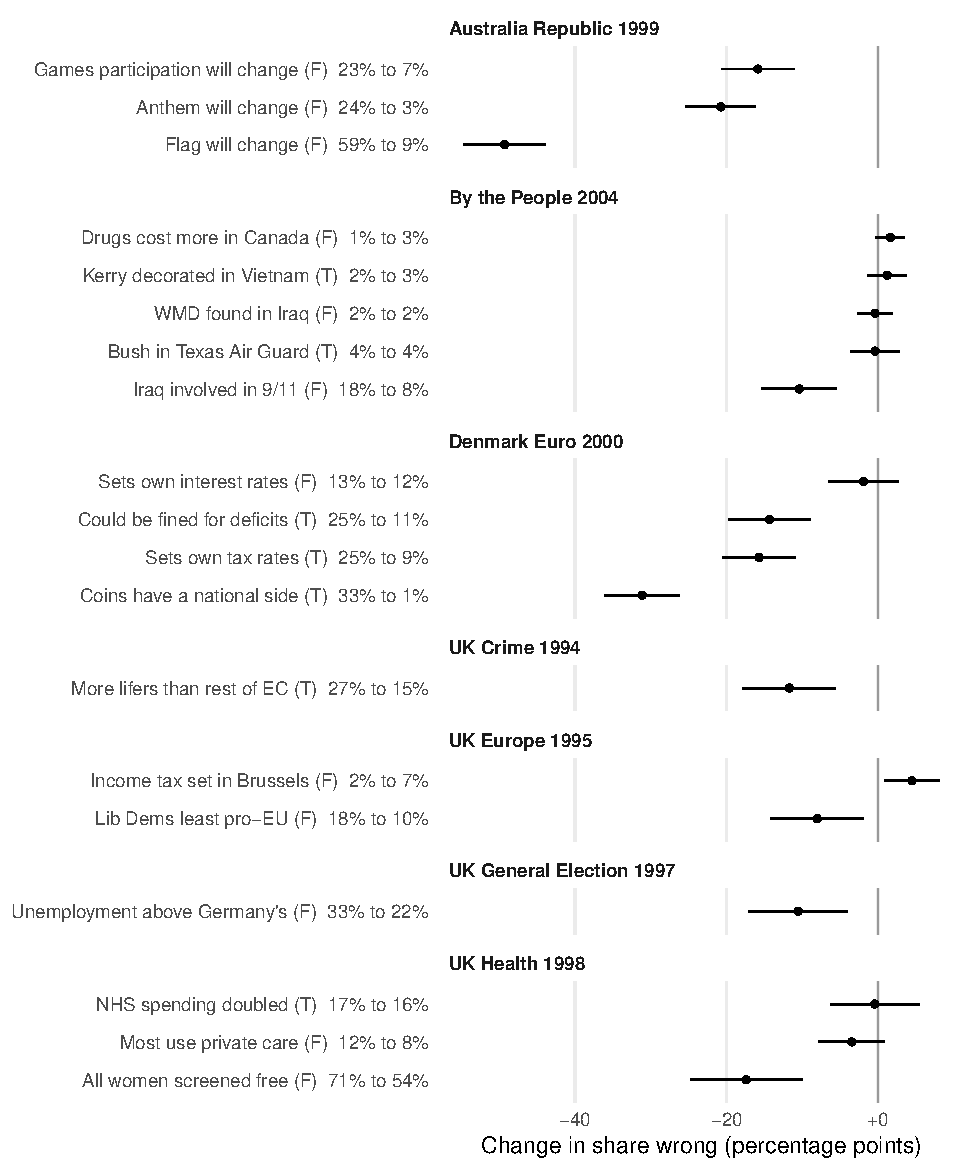
\includegraphics[width=\linewidth]{item_changes.pdf}
\caption{Change in the share of participants answering each item incorrectly between the start and the end of the Deliberative Poll. Labels give the shares before and after; T and F mark true and false statements. Lines are 95\% intervals from the paired differences. Don't know and no answer count as not incorrect.}
\label{fig:items}
\end{figure}

Figure~\ref{fig:items} shows the change on each item. Across the \nItems{} items, the share answering incorrectly fell from \wrongBefore{} to \wrongAfter{}, by \pooledChange{} percentage points (95\% interval \pooledLower{} to \pooledUpper{}). It fell significantly on \nFell{} items and rose significantly on \nRose{}. The largest declines were in the Australian poll: before it, \flagBefore{} of participants thought the flag would definitely change if Australia became a republic; afterward, \flagAfter{} did. The belief that all British women receive free breast screening on the NHS fell only from \screeningBefore{} to \screeningAfter{}, and the belief that Iraq was involved in the September 11 attacks from \iraqBefore{} to \iraqAfter{}. The one rise, in the belief that Britain's income tax rates are decided in Brussels (\brusselsBefore{} to \brusselsAfter{}), is small and on an item that almost everyone answered correctly to begin with.

\subsection{Where Wrong Answers Go}

\begin{figure}[!htbp]
\centering
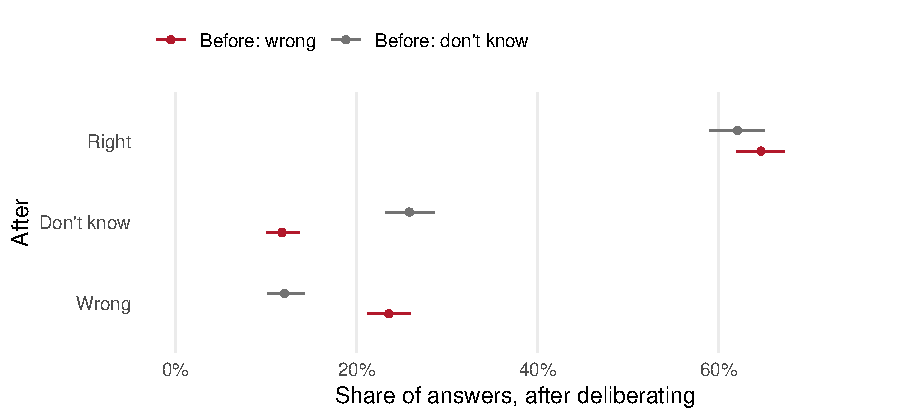
\includegraphics[width=0.85\linewidth]{transitions.pdf}
\caption{Answers at the end of the Deliberative Poll, by answer at the start, pooled over the \nItems{} items (\nStartWrong{} answers wrong at the start, \nStartDk{} without an answer). Lines are 95\% Wilson intervals.}
\label{fig:transitions}
\end{figure}

If misinformation is stubborn, participants who begin with a wrong answer should be harder to move than those who begin with no answer. Figure~\ref{fig:transitions} shows that on the whole they are not. Of answers that were wrong at the start, \wrongToRight{} were right at the end; of answers that were ``don't know'' at the start, \dkToRight{} were. Comparing the two within items, the difference is \rightDiff{} points (95\% interval \rightDiffLower{} to \rightDiffUpper{}). The wrong were not more likely to retreat to ``don't know'' (\wrongToDk{}, against \dkToDk{} of those who began there), but they were twice as likely to end wrong (\wrongToWrong{}, against \dkToWrong{} of those who began without an answer). Only \rightToWrong{} of initially right answers became wrong.

Two readings of this pattern are possible, and the data cannot fully separate them. Many initial wrong answers were probably guesses or weakly held beliefs, easily displaced by what participants heard; the quarter that stayed wrong may be where the misinformation, in the strict sense, lies. Alternatively, wrong answers may reflect engagement with the topic, which also makes learning easier. Either way, deliberation did not leave the wrong answers in place.

\subsection{Comparisons with Control Groups}

\begin{figure}[!htbp]
\centering
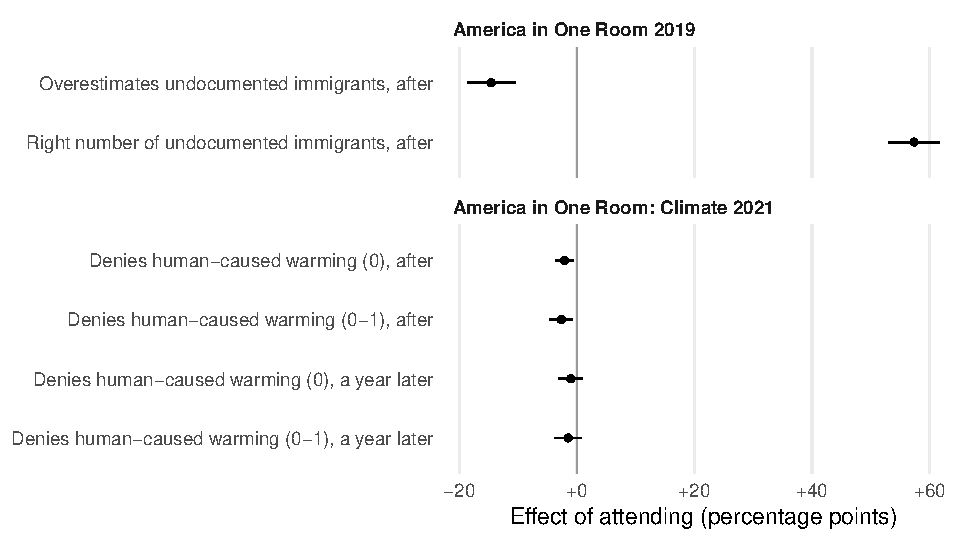
\includegraphics[width=\linewidth]{controlled.pdf}
\caption{Effect of attending on misinformation-type answers in the two Deliberative Polls with control groups: the difference between attendees and controls in the later answer, holding the baseline answer fixed. Lines are 95\% intervals with heteroskedasticity-robust standard errors.}
\label{fig:controlled}
\end{figure}

Without control groups, some of the change above could reflect what participants would have learned anyway, or the effect of answering the same questions twice. The two recent polls address this (Figure~\ref{fig:controlled}). In America in One Room, \immTreatedBefore{} of attendees overestimated the number of undocumented immigrants at the start and \immTreatedAfter{} at the end, while the control group went from \immControlBefore{} to \immControlAfter{}. Holding baseline answers fixed, attending reduced overestimates by \immEffect{} points (95\% interval \immLower{} to \immUpper{}; \immWeighted{} points with the study's weights), and the share giving the right number rose from \rightTreatedBefore{} to \rightTreatedAfter{}. The Danish poll's published comparison groups point the same way: on whether Denmark could be fined for large deficits in the monetary union, correct answers rose from 41 to 80 percent among participants, while 34 percent of the whole recruitment sample and 36 percent of a separate control group surveyed at the end of the event answered correctly \citep[158]{hansen2004}.

Confident denial is harder to move, if only because there is less of it. In the climate edition, \denyTreatedBefore{} of attendees and \denyControlBefore{} of controls rated the statement that warming is human-caused a 0 at the start; afterward, \denyTreatedAfter{} and \denyControlAfter{} did. Attending reduced confident denial by \denyEffect{} points (95\% interval \denyLower{} to \denyUpper{}) and raised average agreement by \agreeEffect{} points on the 0--10 scale. A year later, the effect on denial was \denyLaterEffect{} points (\denyLaterLower{} to \denyLaterUpper{}), no longer distinguishable from zero, though average agreement remained \agreeLaterEffect{} points higher (\agreeLaterLower{} to \agreeLaterUpper{}).

\FloatBarrier
\section{Discussion}

Deliberation dispels much of what looks like misinformation. Across very different polls, countries, and topics, participants gave far fewer incorrect answers at the end than at the start, and those who began wrong were as likely to end right as those who began knowing nothing. This fits the growing evidence that corrections work better than early studies of backfire suggested \citep{wood2019, chan2017}, and it suggests that the richer, two-sided information environment of a Deliberative Poll is an effective vehicle for them.

Three limits bear on how far to take this. First, most of the evidence comes from before-and-after comparisons, which the comparisons with control groups support but cannot validate item by item. Second, incorrect answers are not all misinformation; the one item that measures confidence shows less misinformation to begin with, and less movement, than the others. Where we can isolate confident denial, a weekend of deliberation reduced it only slightly, and the reduction did not clearly last a year. Confident wrong answers may themselves be less stable than they look \citep{graham2023}. Third, the items are those the polls happened to ask. They were not chosen to test misinformation and include few of the beliefs most tied to partisan identity.

The central finding is nonetheless clear. A mistaken belief did not make participants harder to inform. The quarter of wrong answers that persisted is where stubborn misinformation, if it exists in these data, is to be found.

\bibliographystyle{apsr}
\bibliography{references}

\clearpage
\appendix
\section*{Appendix}
\setcounter{table}{0}
\renewcommand{\thetable}{A\arabic{table}}

\begin{table}[H]
\centering
\caption{Misinformation-type items in the seven Deliberative Polls}
\label{tab:items}
\small
\begin{tabular}{lp{10cm}c}
\toprule
Poll & Statement & Key \\
\midrule
UK Crime 1994 & More people are serving life sentences in Britain than in the rest of the European Community put together & T \\
UK Europe 1995 & Britain's income tax rates are decided in Brussels & F \\
 & Of the three British parties, the Liberal Democrats are least in favour of the European Union & F \\
UK General Election 1997 & Unemployment in Britain is higher than in Germany & F \\
UK Health 1998 & Even with inflation taken into account, spending on the NHS has doubled over the last 20 years & T \\
 & Most people use private medical treatment instead of the NHS & F \\
 & All British women get free breast cancer screening on the NHS & F \\
Australia Republic 1999 & If Australia becomes a republic, the flag will definitely change & F \\
 & If Australia becomes a republic, the national anthem will definitely change & F \\
 & If Australia becomes a republic, participation in the Commonwealth Games will definitely change & F \\
Denmark Euro 2000 & As a member of the monetary union, Denmark could be fined if its deficit is too large & T \\
 & Denmark can decide its own interest rates if it joins the monetary union & F \\
 & Denmark can decide its own rates of taxation if it joins the single currency & T \\
 & The euro coins will have a national side & T \\
By the People 2004 & Iraq was directly involved in the attacks on the World Trade Center and the Pentagon on 9/11 & F \\
 & Large quantities of weapons of mass destruction have been found in Iraq & F \\
 & On average, prescription drugs cost more in Canada than in the U.S. & F \\
 & During the Vietnam War, George W. Bush served in the Texas Air National Guard & T \\
 & During the Vietnam War, John Kerry was a decorated officer serving in Vietnam & T \\
\bottomrule
\end{tabular}

\begin{minipage}{0.9\linewidth}
\vspace{0.5em}\footnotesize \emph{Note:} T and F give whether the statement is true or false. The Vietnam items were multiple choice; the statement is the correct option. Sources for each key are in the replication files.
\end{minipage}
\end{table}

\end{document}
